\section{Lógica Fuzzy}
\subsection{Conceito}
Também chamada de \textit{Lógica Nebulosa}, ela permite a utilização de graus de pertinência entre 
$[0, 1]$ em vez de decisões puramente binárias. Em outras palavras, em vez de classificar algo 
apenas como ``verdadeiro'' ou ``falso'', ela admite níveis intermediários — como tons de cinza entre 
o preto e o branco. Tomando-se como exemplo um dia  
em que a temperatura está marcando $27\degree$: ele é um dia quente ou um dia frio? Bom, a resposta 
vai variar dependendo de para quem se faz essa pergunta. Para alguém do Ceará, 
por exemplo, provavelmente é um dia frio, porém, para alguém  
do Rio Grande do Sul, provavelmente será o contrário.

Nesse contexto, em vez de tentar rotular estritamente 
$27\degree$ como quente ($0$) ou frio ($1$) como na lógica binária, a lógica fuzzy daria o grau de pertinência 
da categoria quente e da categoria frio, ou seja, quanto essa temperatura pode ser considerada quente ao 
mesmo tempo de quanto que essa temperatura pode ser considerada fria. Assim, a partir desse exemplo, 
é possível retirar alguns conceitos:

\begin{itemize}
    \item \emph{Variável Fuzzy:} É o nome dado àquilo que está sendo avaliado — no exemplo, seria ``temperatura'';
    \item \emph{Conjunto linguístico:} São os ``adjetivos'' que podem ser atribuídos à variável fuzzy — no exemplo, 
    seria [quente, frio], mas poderiam haver mais ``adjetivos'', por exemplo, [muito quente, quente, agradável, frio, muito frio];
    \item \emph{Função de pertinência:} converte os valores das variáveis numéricas em graus de pertinência da variável fuzzy equivalente.
\end{itemize}

Agora, com a lógica devidamente explicada, é possível descrever a ideia por trás de um \emph{controlador fuzzy}. 
Sua estrutura é composta por quatro etapas: fuzzificação (conversão de entradas numéricas em graus 
de pertinência por funções de pertinência), base de regras (relações do tipo ``se–então'' que conectam 
entradas e saídas), inferência fuzzy (combinação das regras acionadas, por exemplo, pelo método de 
Mamdani) e defuzzificação (conversão do resultado fuzzy em um valor numérico, por exemplo, pelo 
método do centro de gravidade).

Além disso, em sistemas MIMO, cada variável de entrada pode gerar 
múltiplas combinações fuzzy, aumentando o número de regras. Assim, o desempenho do controlador 
depende fortemente do desenho das funções de pertinência e da formulação adequada da base de 
regras, que determinam a resposta dinâmica do sistema.

\subsection{Implementação}
A Figura \ref{fig:pid_diagram} esquematiza o controlador fuzzy que foi desenvolvido neste trabalho cuja 
implementação foi feita em Python, utilizando as bibliotecas \texttt{scikit-fuzzy} e \texttt{SciPy}. 
\begin{figure}[h!]
    \centering
    \caption{Diagrama de Blocos do Controlador fuzzy para o Drone.}
    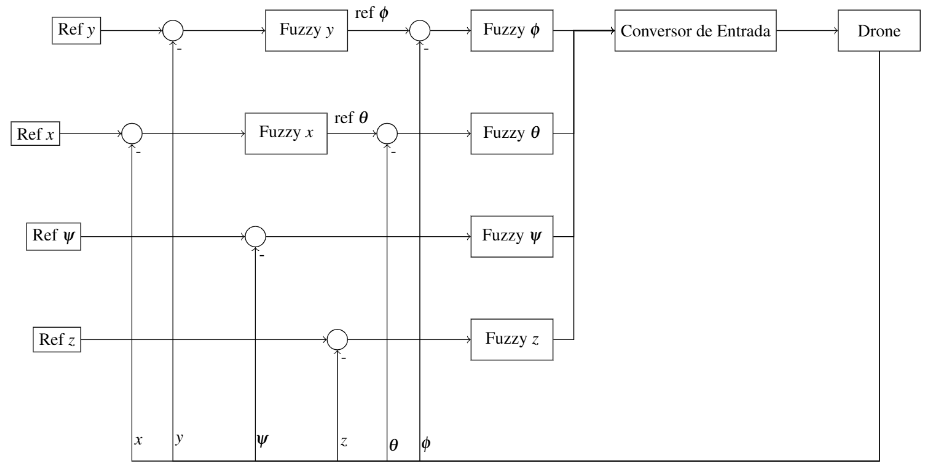
\includegraphics[width=0.9\textwidth]{figs/fuzzy_drone.png}
    \label{fig:pid_diagram}
\end{figure}

\pagebreak

Como o drone é simétrico, os controladores de $\phi$ e $\theta$, bem como os de $x$ e $y$, 
compartilham, respectivamente, as mesmas funções de pertinência. Por fim, foram definidas duas 
entradas para cada controlador — $E_i$ (erro em $i$) e $V_i$ (velocidade em $i$) —, bem como uma 
saída — $U_i$ (saída de controle em $i$). A Tabela \ref{tab:func_pert} agrupa todas as funções de pertinência 
utilizadas neste trabalho.

\begin{table}[h!]
\centering
\begin{tabular}{|c|c|c|c|c|c|}
    \hline
    Variável & Conjunto Linguístico & Função de Pertinência & Começo & Pico & Fim \\
    \hline
    $E_x$ & $--$ & Triangular & -10 & -10 & -1 \\
    $E_x$ & $-$  & Triangular & -10 & -1 & 0 \\
    $E_x$ & $0$  & Triangular & -1 & 0 & 1 \\
    $E_x$ & $+$  & Triangular & 0 & 1 & 10 \\
    $E_x$ & $++$ & Triangular & 1 & 10 & 10 \\
    \hline
    $E_{z}$ & $--$ & Triangular & -10 & -10 & -0.01 \\
    $E_{z}$ & $-$  & Triangular & -10 & -0.01 & 0 \\
    $E_{z}$ & $0$  & Triangular & -0.01 & 0 & 0.01 \\
    $E_{z}$ & $+$  & Triangular & 0 & 0.01 & 10 \\
    $E_{z}$ & $++$ & Triangular & 0.01 & 10 & 10 \\
    \hline
    $E_{\phi}$ & $--$ & Triangular & -15 & -15 & -0.1 \\
    $E_{\phi}$ & $-$  & Triangular & -15 & -0.1 & 0 \\
    $E_{\phi}$ & $0$  & Triangular & -0.1 & 0 & 0.1 \\
    $E_{\phi}$ & $+$  & Triangular & 0.1 & 0.1 & 15 \\
    $E_{\phi}$ & $++$ & Triangular & 0.1 & 15 & 15 \\
    \hline
    $E_{\psi}$ & $--$ & Triangular & -45 & -45 & -0.1 \\
    $E_{\psi}$ & $-$  & Triangular & -45 & -0.1 & 0 \\
    $E_{\psi}$ & $0$  & Triangular & -0.1 & 0 & 0.1 \\
    $E_{\psi}$ & $+$  & Triangular & 0.1 & 0.1 & 45 \\
    $E_{\psi}$ & $++$ & Triangular & 0.1 & 45 & 45 \\
    \hline
\end{tabular}

\caption{Funções de Pertinência do erro $E$.}
\label{tab:fuzzy_error}
\end{table}


\begin{table}[h!]
\centering
\begin{tabular}{|c|c|c|c|c|c|}
    \hline
    Variável & Conjunto Linguístico & Função de Pertinência & Começo & Pico & Fim \\
    \hline
    $V_x$ & $-$ & Triangular & -5 & -5 & -0 \\
    $V_x$ & $0$  & Triangular & -5 & 0 & 5 \\
    $V_x$ & $+$ & Triangular & 0 & 5 & 5 \\
    \hline
    $V_{z}$ & $-$  & Triangular & -50 & -50 & 0 \\
    $V_{z}$ & $0$  & Triangular & -50 & 0 & 50 \\
    $V_{z}$ & $+$  & Triangular & 0 & 50 & 50 \\
    \hline
    $V_{\phi}$ & $-$  & Triangular & -20 & -20 & 0 \\
    $V_{\phi}$ & $0$  & Triangular & -20 & 0 & 20 \\
    $V_{\phi}$ & $+$  & Triangular & 20 & 30 & 20 \\
    \hline
    $V_{\psi}$ & $-$  & Triangular & -20 & -20 & 0 \\
    $V_{\psi}$ & $0$  & Triangular & -20 & 0 & 20 \\
    $V_{\psi}$ & $+$  & Triangular & 20 & 20 & 20 \\
    \hline
\end{tabular}
\caption{Funções de Pertinência da velocidade $V$.}
\label{tab:fuzzy_error}
\end{table}


\begin{table}[h!]
\centering
\begin{tabular}{|c|c|c|c|c|c|}
    \hline
    Variável & Conjunto Linguístico & Função de Pertinência & Começo & Pico & Fim \\
    \hline
    $U_x$ & $--$ & Triangular & -20 & -20 & -10 \\
    $U_x$ & $-$  & Triangular & -20 & -10 & 0 \\
    $U_x$ & $0$  & Triangular & -10 & 0 & 10 \\
    $U_x$ & $+$  & Triangular & 0 & 10 & 20 \\
    $U_x$ & $++$ & Triangular & 10 & 20 & 20 \\
    \hline
    $U_{z}$ & $--$ & Triangular & -100 & -100 & -50 \\
    $U_{z}$ & $-$  & Triangular & -100 & -50 & 0 \\
    $U_{z}$ & $0$  & Triangular & -50 & 0 & 50 \\
    $U_{z}$ & $+$  & Triangular & 0 & 50 & 100 \\
    $U_{z}$ & $++$ & Triangular & 50 & 100 & 100 \\
    \hline
    $U_{\phi}$ & $--$ & Triangular & -100 & -100 & -30 \\
    $U_{\phi}$ & $-$  & Triangular & -100 & -30 & 0 \\
    $U_{\phi}$ & $0$  & Triangular & -30 & 0 & 30 \\
    $U_{\phi}$ & $+$  & Triangular & 30 & 30 & 100 \\
    $U_{\phi}$ & $++$ & Triangular & 30 & 100 & 100 \\
    \hline
    $U_{\psi}$ & $--$ & Triangular & -100 & -100 & -50 \\
    $U_{\psi}$ & $-$  & Triangular & -100 & -50 & 0 \\
    $U_{\psi}$ & $0$  & Triangular & -50 & 0 & 50 \\
    $U_{\psi}$ & $+$  & Triangular & 50 & 50 & 100 \\
    $U_{\psi}$ & $++$ & Triangular & 50 & 100 & 100 \\
    \hline
\end{tabular}
\caption{Funções de Pertinência do Entrada do Sistema $U$.}
\label{tab:fuzzy_error}
\end{table}

Por fim, seguem abaixo as regras implementadas nos controladores fuzzy:
\vspace{-0.3cm}
\begin{equation*}
\begin{aligned}
    &\text{1. } \textit{if } E \textit{ is } ++ \textit{ then } U \textit{ is } ++, \\
    &\text{2. } \textit{if } E \textit{ is } + \textit{ and } V \textit{ is } + \textit{ then } U \textit{ is } -, \\
    &\text{3. } \textit{if } E \textit{ is } + \textit{ and } V \textit{ is } - \textit{ then } U \textit{ is } +, \\
    &\text{4. } \textit{if } E \textit{ is } 0 \textit{ then } U \textit{ is } 0, \\
    &\text{5. } \textit{if } E \textit{ is } - \textit{ and } V \textit{ is } - \textit{ then } U \textit{ is } +, \\
    &\text{6. } \textit{if } E \textit{ is } - \textit{ and } V \textit{ is } + \textit{ then } U \textit{ is } -, \\
    &\text{7. } \textit{if } E \textit{ is } -- \textit{ then } U \textit{ is } --.
\end{aligned}
\end{equation*}

% \subsection{Resultados}